\begin{figure}[htbp]
    \centering
    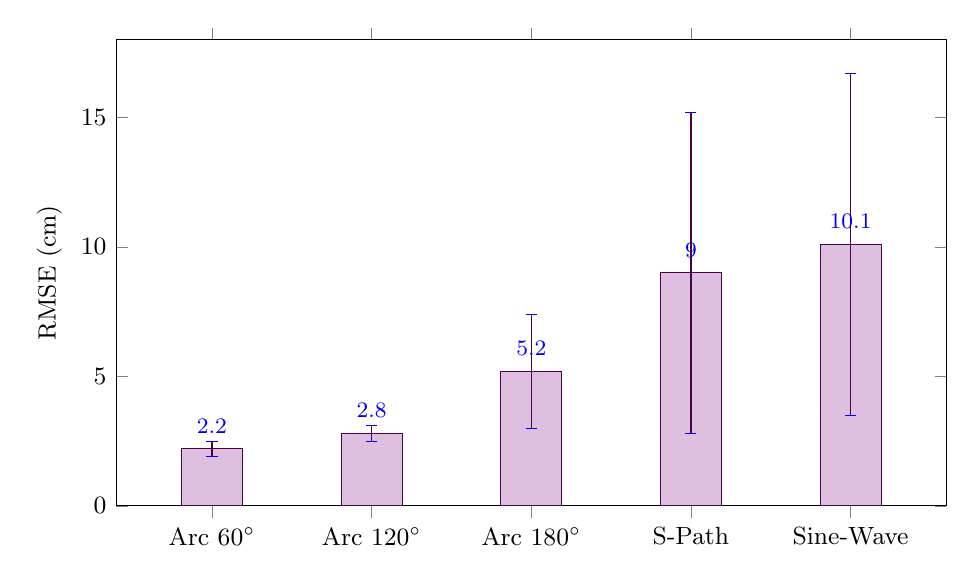
\begin{tikzpicture}
    \begin{axis}[
        ybar,
        bar width=22pt,
        width=\textwidth, height=7.5cm,
        enlarge x limits=0.15,
        ymin=0, ymax=18,
        ylabel={RMSE (cm)},
        symbolic x coords={Arc 60$^\circ$, Arc 120$^\circ$, Arc 180$^\circ$, S-Path, Sine-Wave},
        xtick={Arc 60$^\circ$, Arc 120$^\circ$, Arc 180$^\circ$, S-Path, Sine-Wave},
        error bars/y dir=both, error bars/y explicit,
        tick label style={font=\small},
        label style={font=\small},
        nodes near coords,
        nodes near coords style={font=\footnotesize},
        every node near coord/.append style={yshift=2pt},
    ]
    \addplot+[draw=violet!60!black, fill=violet!25] coordinates {
        (Arc 60$^\circ$,2.2) +- (0,0.3) (Arc 120$^\circ$,2.8) +- (0,0.3)
        (Arc 180$^\circ$,5.2) +- (0,2.2) (S-Path,9.0) +- (0,6.2)
        (Sine-Wave,10.1) +- (0,6.6) };
    \end{axis}
    \end{tikzpicture}
    \caption[Path generalization of the pushing policy]{Bar-chart visualization of the path-generalization results reported in \cref{tab:pho_paths} for the pushing-heavy-objects policy. Bars show tracking RMSE under novel path geometries with in-distribution physical parameters; error bars denote one standard deviation. Tracking error degrades gracefully as path curvature complexity increases.}
    \label{fig:pho_paths_bars}
\end{figure}
